\documentclass[a4paper,twoside,master.tex]{subfiles}
\begin{document}
\lecture{17}{Friday, February 21, 2020}{Maxwell Relations}

From last lecture, we decided we don't really care about the number of particles, and we can write partial derivatives in terms of Jacobians:
\begin{equation}
    \eval{\pdv{P}{T}}_{V,N} \equiv \eval{\pdv{P}{T}}_{V} = \pdv{(P,V)}{(T,V)} = \pdv{(P,V)}{\color{red}(P,T)\color{black}} \pdv{\color{red}(P,T)\color{black}}{(T,V)}
\end{equation}

Typically, we want to introduce a Jacobian made of the variables used in the original derivative (in this case, $ P $ and $ T $). It usually makes for a simple transformation, but it is obviously not the only possibility. For the magic to work out, we need things to be in the same ``slot'', and switching ordering means introducing minus signs:
\begin{equation}
    - \pdv{(V,P)}{(T,P)} \pdv{(P,T)}{\color{red}(V,T)\color{black}} = - \eval{\pdv{V}{T}}_{P} \eval{\pdv{P}{V}}_{T}
\end{equation}

We can then use inverses:
\begin{equation}
    - \eval{\pdv{V}{T}}_{P} \eval{\pdv{P}{V}}_{T} = \frac{\frac{1}{V} \eval{\pdv{V}{T}}_{P}}{- \frac{1}{V} \eval{\pdv{V}{P}}_{T}} = \frac{\alpha}{K_T}
\end{equation}

\section{The Joule-Thomson Effect}
\label{sec:the_joule-thomson_effect}
\begin{figure}[h]
    \centering
    \includegraphics[width=\textwidth/2]{figures/lec_17_joule_thomson.png}
    \caption{Demonstration of the Joule-Thomson Effect}
    \label{fig:joule_thomson}
\end{figure}
Fun fact, Thomson is William Thomson, aka Kelvin. Let's imagine a container with two pistons (see \Cref{fig:joule_thomson}). The gas in compartment $ A $ is at pressure $ P_A $ and the gas in $ B $ is at $ P_B $. Suppose we start with $ P_A > P_B $ and we maintain this while moving the pistons such that the gas moves from compartment $ A $ to compartment $ B $. The energy in $ B $ can be written
\begin{equation}
    U_B = U_A + P_A V_A - P_B V_B
\end{equation}
Note that this implies the enthalpy stays constant (isenthalpic process):
\begin{equation}
    H_A = U_A + P_A V_A = U_B + P_B V_B = H_B
\end{equation}

How does the temperature of the gas change? For a small pressure difference at constant $ N $ and $ H $, we have
\begin{equation}
    \dd{T} = \eval{\pdv{T}{P}}_{H,N} \dd{P} = \mu_{\text{JT}}
\end{equation}
where $ \mu_{\text{JT}} $ is the ``Joule-Thomson coefficient''. If $ \mu_{\text{JT}} > 0 $, the gas cools in the process. Let's use Maxwell relations to transform this into something we can measure:

\begin{equation}
    \mu_{\text{JT}} = \eval{\pdv{T}{P}}_{H,N} = \pdv{(T,H)}{P,H} = -\pdv{(T,H)}{(T,P)} \pdv{(T,P)}{(H,P)} = - \frac{\eval{\pdv{H}{P}}_{T}}{\eval{\pdv{H}{T}}_{P}}
\end{equation}

Next, let's work out what these derivatives are. Recall the enthalpy $ H(S,P,N) $ has a differential form:
\begin{equation}
    \dd{H} = T \dd{S} + V \dd{P} + \mu \dd{N}
\end{equation}
We agreed at doing this at constant $ N $, so we really only need $ \dd{H} = T \dd{S} + V \dd{P} $.
\begin{equation}
    \eval{\pdv{H}{P}}_{T} = T \eval{\pdv{S}{P}}_{T} + V \eval{\pdv{P}{T}}_{T}
\end{equation}

We can justify this with the chain rule:
\begin{align}
    \eval{\pdv{H(S,P,N)}{P}}_{T,N} &= \eval{\pdv{H}{S}}_{P,N} \eval{\pdv{S}{P}}_{T,N} + \eval{\pdv{H}{P}}_{S,N} \eval{\pdv{P}{P}}_{T,N} + \eval{\pdv{H}{N}}_{S,P} \eval{\pdv{N}{P}}_{T,N} \\
    &= T \eval{\pdv{S}{P}}_{T,N} + V \eval{\pdv{P}{P}}_{T,N} + \mu \eval{\pdv{N}{P}}_{T,N}
\end{align}

\begin{equation}
    \pdv{P}{P} = 1
\end{equation}
so we really only need to find
\begin{equation}
    \eval{\pdv{S}{P}}_{T} = -\eval{\pdv{V}{T}}_{P}
\end{equation}
using Maxwell's relations.

How does the volume change while keeping the pressure fixed? This is typically thought of as the thermal expansion, but we need that $ \frac{1}{V} $ factor to make it into the defined material property:
\begin{equation}
    \eval{\pdv{H}{P}}_{T}  = -TV \frac{1}{V} \eval{\pdv{V}{T}}_{P} + V = V(1-T \alpha)
\end{equation}

Now for the denominator:
\begin{equation}
    \eval{\pdv{H}{T}}_{P} = T \eval{\pdv{S}{T}}_{P} + V \eval{\pdv{P}{T}}_{P} + \left( \dd{N} \text{ stuff} \right) = N \frac{T}{N} \eval{\pdv{S}{T}}_{P} = NC_p
\end{equation}

Therefore,
\begin{equation}
    \mu_{\text{JT}} = - \frac{V(1-T \alpha)}{NC_P} = - \frac{V}{NC_P} (T \alpha - 1)
\end{equation}

What happens when we do this with an ideal gas?
\begin{equation}
    \alpha = \frac{1}{V} \eval{\pdv{V}{T}}_{P} = \frac{1}{V} \pdv{T} \left( \frac{N k_B T}{P} \right) = \frac{1}{V} \frac{N k_B}{P} = \frac{1}{T}
\end{equation}

Therefore, $ \mu_{\text{JT}, \text{ideal}} = 0 $!\ We can't use ideal gasses to enact the Joule-Thomson effect to cool or heat a gas.

\end{document}
